%type de document
\documentclass[a4paper,12pt]{article}

% r�gles typographiques fran�aises
\usepackage[latin1]{inputenc}
\usepackage[francais]{babel}
\usepackage[T1]{fontenc}


% mise en page
\usepackage[margin=2.5cm]{geometry}
\usepackage{fancyhdr}
\usepackage{graphicx}
\usepackage{array}
\usepackage{lastpage}
\usepackage{placeins}
\usepackage{longtable}
\usepackage{caption}
\usepackage{float}
\usepackage{wrapfig}
\usepackage{dirtree}

\usepackage[smaller, footnote, printonlyused]{acronym} % table d'acronymes, option [footnote] pour avoir les d�finitions en bas de page [printonlyused

\usepackage{hyperref}
\hypersetup{colorlinks=true, linkcolor=blue}
\hypersetup{pdfauthor=Sebastien Chassot}
\hypersetup{pdfstartpage=1}
\hypersetup{pdfpagemode=None} %FullScreen, None
\hypersetup{pdfpagelayout=SinglePage} %SinglePage, OneColumn, TwoColumnLeft, TwoColumnRight
\hypersetup{pdfstartview=FitH} %Fit, FitH, FitV, FitB, FitBH, FitBV
\pdfcompresslevel=9
%\hypersetup{
%  bookmarks=true                % show bookmarks bar?
%, bookmarksopen=true
%, unicode=false                 % non-Latin characters in Acrobat bookmarks
%, pdftoolbar=true               % show Acrobat toolbar?
%, pdfmenubar=true               % show Acrobat menu?
%, pdffitwindow=false            % window fit to page when opened
%, pdfpagemode=UseOutlines       % FullScreen, UseThumbs(show thumbnails)
%                                % UseOutlines(show bookmarks), None
%, pdfpagelayout=SinglePage      % SinglePage, OneColumn, TwoColumnLeft, TwoColumnRight
%, pdfstartpage=1
%, pdfstartview={FitV}           % Fit, FitH, FitV, FitB, FitBH, FitBV
%, pdfsubject={}
%, pdftitle={Rapport}    		% title
%, pdfauthor={J. Mendes, S. Chassot, D. Wittwer}       	% author
%, pdfcreator={LaTeX}            % creator of the document
%, pdfkeywords={HEPIA} {Rapport} {analyse} {programmation} {terminal} {c}  % list of keywords
%, pdfnewwindow=true             % links in new window
%, colorlinks=false              % false: boxed links; true: colored links
%, linkcolor=red                 % color of internal links
%, citecolor=black               % color of links to bibliography
%, filecolor=magenta             % color of file links
%  urlcolor=blue                 % color of external links
%}

% Espacement interligne
\usepackage{setspace}
\onehalfspacing

% Couleur
\usepackage{colortbl}
\definecolor{bleuClair}{rgb}{0.31,0.51,0.74}

% ligne vide
\newcommand{\emptyLine}[1][1]{\par\leavevmode\par}

% lstlisting configuration
\usepackage{fancyvrb}
\usepackage{xcolor}
\usepackage{listings}

% D�finition des couleurs
\definecolor{lightgreen}{rgb}{0.2,.98,0.2}
\definecolor{darkgreen}{rgb}{0,0.4,0}
\definecolor{lightgray}{gray}{0.98}
\definecolor{darkred}{rgb}{0.545,0.000,0.000}
\definecolor{bleuClair}{rgb}{0.31,0.51,0.74}
\definecolor{grisTableau}{rgb}{0.9529,0.9529,0.9529}
\lstset {	
  language=C
, frame=single
, keepspaces=true
, columns=fullflexible
, captionpos=b
, stepnumber=10
, morekeywords={var,get,set}
, basicstyle=\ttfamily\scriptsize
, keywordstyle=\color{blue}
, commentstyle=\color{darkgreen}
, stringstyle=\color{darkred}
, backgroundcolor=\color{white}
, numbers=left
, numberstyle=\scriptsize
, numbersep=5pt
, breaklines=true
, tabsize=3
, showstringspaces=false
, emph={double,bool,int,unsigned,char,true,false,void,get,set}
, emphstyle=\color{blue}
, emph={Assert,Test}
, emphstyle=\color{red}
, emph={[2]\#using,\#define,\#ifdef,\#endif}
, emphstyle={[2]\color{blue}}
, rulesepcolor=\color{gray}
, lineskip={-1.5pt} % single line spacing
, escapeinside={/*(*@}{@*)*/}
, rangeprefix=\{\  % curly left brace plus space
, rangesuffix=\ \} % space plus curly right brace
}
\lstset{prebreak=\raisebox{0ex}[0ex][0ex]
        {\ensuremath{\hookleftarrow}}}
%\lstset{postbreak=\raisebox{0ex}[0ex][0ex]
%        {\ensuremath{\hookrightarrow\space}}}
\lstset{breaklines=true, breakatwhitespace=true}

% replace sequence of char by another sequence of char
% see http://stackoverflow.com/questions/1116266/listings-in-latex-with-utf-8-or-at-least-german-umlauts
\lstset{literate=%
{ä}{{\"a}}1
{â}{{\^a}}1
{� }{{\`a}}1
{ë}{{\"e}}1
{ê}{{\^e}}1
{é}{{\'e}}1
{è}{{\`e}}1
{ï}{{\"i}}1
{î}{{\^i}}1
{ö}{{\"o}}1
{ô}{{\^o}}1
{ü}{{\"u}}1
{û}{{\^u}}1
{ç}{{\c c}}1
{°}{{\textsuperscript{o}}}1
% suppress BOM (Byte Order Mark) characters at the beginning of Visual Studio source
% see http://tex.stackexchange.com/questions/5935/how-to-suppress-bom-effect-in-the-output
{�}{}0
{�}{}0
{�}{}0
}

%%%%%%%%%%%%%%%%%%%%%%%%%%%%%%%%%%%%%%%%%%%%%%%%%%%%%%%%%%%%%%%%%
%		DEBUT DU DOCUMENT
%%%%%%%%%%%%%%%%%%%%%%%%%%%%%%%%%%%%%%%%%%%%%%%%%%%%%%%%%%%%%%%%%

\begin{document}

%%%%%%%%%%%%%%%%%%%%%%%%%%%%%%%%%%%%%%%%%%%%%%%%%%%%%%%%%%%%%%%%%%%
%		ENTETE ET PIED DE PAGE
%%%%%%%%%%%%%%%%%%%%%%%%%%%%%%%%%%%%%%%%%%%%%%%%%%%%%%%%%%%%%%%%%
\pagestyle{fancy}
% ent�te
\lhead{}
\chead{}
\rhead{}
% pied de page
\lfoot{}
\cfoot{Page \thepage\ sur \pageref{LastPage} }
\rfoot{}
\renewcommand{\headrulewidth}{0.1pt}
\renewcommand{\footrulewidth}{0.1pt}
\fancyhead[R]{\textsl{ prog system - TP Minix File system }}
%\fancyfoot[C]{\scriptsize\emph{\class}}

\fancyfoot[L]{\scriptsize\emph{\docschool{}}}


%%%%%%%%%%%%%%%%%%%%%%%%%%%%%%%%%%%%%%%%%%%%%%%%%%%%%%%%%%%%%%%%%%%

\author{Sebastien Chassot, Andre-Luc Rrobyr}
\newcommand{\docschool}{hepia - ITI}
\title{Rapport}

% page de titre
\begin{center}
\includegraphics[scale=2]{imgs/hepia}
\end{center}

\vspace{3cm}

\begin{center}
\begin{huge}
\textbf{Rapport}
\end{huge}
\end{center}

\begin{center}
\begin{large}
Minix File system
\end{large}
\end{center}

% Trait de separation
\newcommand{\lineunder}{\color{bleuClair}\hrulefill\\\color{black}}
\lineunder

\begin{center}
\begin{large}
ITI 2\up{�me} soir \\
2014 / 2015
\end{large}
\end{center}

\vspace{3cm}
\centerline{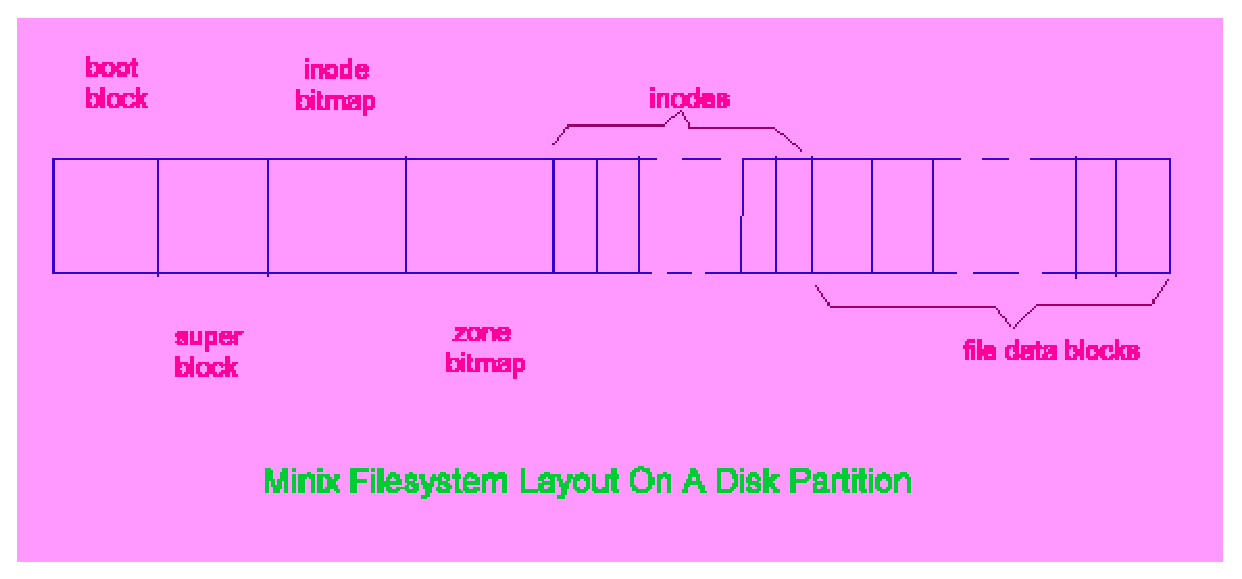
\includegraphics[scale=0.4]{imgs/fs6}}
\vspace{2cm}

\begin{center}
%\begin{large}
\textbf{Sebastien Chassot, Andre-Luc Rrobyr} \\ Juin 2015
%\end{large}
\end{center}

\thispagestyle{empty} % enleve les entetes et pide de page de la page de titre

% table des mati�res
\newpage % nouvelle page
\tableofcontents % table des mati�res
\newpage % nouvelle page

%\chapter*{Mini Bash}


\section{Introduction}



\vspace{1cm}

\section{Le serveur de blocs}

\subsection*{la probl�matique de la d�connexion du client}

D�tecter la d�connexion d'un client n'est pas trivial. En effet, lors d'un \emph{shutdown()}, 


\subsection*{Solutions envisag�es}

Une des solutions les plus simple serait de traiter un �change � la fois; le client se connecte, envoit une requ�te, re�oit la r�ponse et se d�connecte. Le server fait la m�me chose; attend sur \emph{accept()} qu'un client se connecte, attend une requ�te y r�pond et se d�connecte.\\

Cette solution est simple, permet de mieux ma�triser l'�tat du client et du server mais est couteuse en connexions.\\

Une autre solution est d'accepter un client et rentrer dans une boucle, un \emph{fork()} ou un thread et traiter les requ�tes du client tant qu'il ne se d�connecte pas. Cette solution est plus �l�gante mais elle n�cessite de d�tecter la d�connexion du client.\\

Une alternative possible est d'ajouter au protocole une requ�te (un message) de d�connexion qui synchronise le client et le server.


 
\end{document} 